\documentclass[tikz,border=8pt]{standalone}
\usepackage{amsmath,amssymb}
\usetikzlibrary{arrows.meta,calc,decorations.markings,decorations.pathmorphing,patterns,shapes.geometric,positioning}

\begin{document}
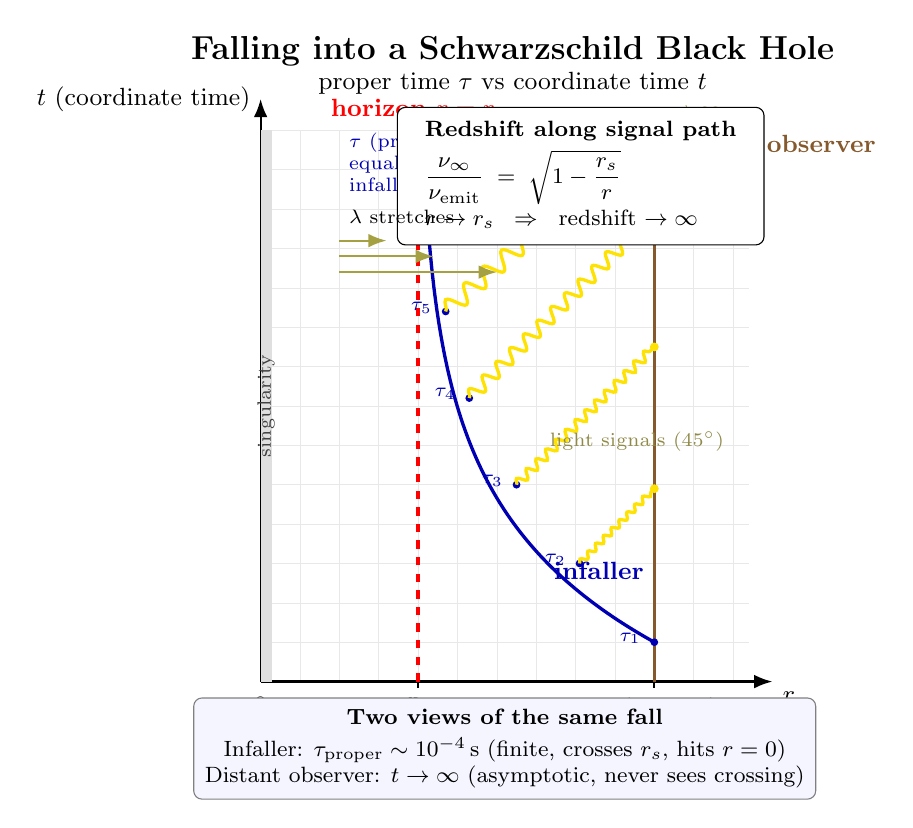
\begin{tikzpicture}[>=Latex,
    scale=1.0,
    every node/.style={font=\small}]

  % --- coordinate frame ---------------------------------------------------
  % horizontal r-axis from 0 to 6, vertical t-axis from 0 to 7
  % horizon at r = 2 (i.e., r_s)

  % background grid (very faint)
  \draw[gray!18, very thin, step=0.5] (0,0) grid (6.2,7.0);

  % axes
  \draw[->, thick] (0,0) -- (6.5,0) node[below right, font=\small] {$r$};
  \draw[->, thick] (0,0) -- (0,7.4) node[left, font=\small] {$t$ (coordinate time)};

  % tick marks on r-axis
  \draw[thick] (2,0.05) -- (2,-0.08) node[below, font=\small] {$r_s$};
  \draw[thick] (5,0.05) -- (5,-0.08) node[below, font=\small] {$r_0$ (distant)};
  \node[below, font=\small] at (0,-0.08) {$0$};

  % --- horizon: vertical dashed red line at r = r_s = 2 -------------------
  \draw[red, very thick, dashed] (2,0) -- (2,7.0)
    node[above, red, font=\small\bfseries] {horizon $r=r_s$};

  % singularity strip
  \fill[gray!25] (0,0) rectangle (0.15, 7.0);
  \node[gray!50!black, font=\scriptsize, rotate=90] at (0.07, 3.5) {singularity};

  % --- distant observer worldline: vertical brown line at r = r_0 = 5 -----
  \draw[brown!70!black, very thick] (5,0) -- (5,7.0);
  \node[brown!70!black, font=\small\bfseries, anchor=south west] at (5.05, 6.6) {distant observer};
  \node[brown!70!black, font=\scriptsize] at (5.0, -0.45) {$r=r_0$};

  % --- infaller worldline: starts at (5, 0.5), curves toward r=2 asymptotically
  % use a smooth curve that approaches r=2 vertically (asymptote)
  \draw[blue!70!black, very thick]
    plot[smooth, samples=100, domain=0.5:6.8] (
       {2 + 3*exp(-0.6*(\x-0.5))},
       {\x}
    );
  \node[blue!70!black, font=\small\bfseries, anchor=west] at (3.6, 1.4) {infaller};

  % proper-time tick marks along the infaller (small marks perpendicular)
  % we mark a few points: tau = tau1, tau2, tau3, tau4 along blue curve
  % spacing in tau is even, but in coordinate time t (=\x), proper-time
  % markers cluster increasingly toward the horizon. We place by hand:
  \foreach \taux/\tauy/\tlabel in {
    5.0/0.5/$\tau_1$,
    4.05/1.5/$\tau_2$,
    3.25/2.5/$\tau_3$,
    2.65/3.6/$\tau_4$,
    2.35/4.7/$\tau_5$
  } {
    \fill[blue!70!black] (\taux,\tauy) circle (1.4pt);
    \node[blue!70!black, anchor=east, font=\scriptsize] at (\taux-0.05, \tauy+0.05) {\tlabel};
  }

  % proper time legend
  \node[blue!70!black, font=\scriptsize, align=left, anchor=west]
    at (1.0, 6.6) {$\tau$ (proper time):\\equal ticks of\\infaller's clock};

  % --- light signals: 45-degree lines from infaller to distant observer ---
  % We send a few photons. Light cones in Schwarzschild are non-trivial,
  % but for visualization we use approximate 45-degree slope outside horizon.
  % Each photon emitted at increasing t from the infaller; arrives at r=5 later.

  % helper: photon paths drawn as wavy yellow lines (decorate snake)
  \tikzset{photon/.style={yellow!85!orange, very thick,
                          decorate, decoration={snake, amplitude=1.0pt, segment length=4pt}}}

  % photon 1: emitted near tau1 (r=5, t=0.5) to r=5 ... trivial (already at observer)
  % photon 2: emitted at (4.05, 1.5), arrives at (5, 2.45)  -- short delay, normal wavelength
  \draw[photon] (4.05,1.5) -- (5.0,2.45);
  \fill[yellow!85!orange] (5.0,2.45) circle (1.6pt);

  % photon 3: emitted at (3.25, 2.5), arrives at (5, 4.25) -- longer
  \draw[photon, decoration={snake, amplitude=1.6pt, segment length=5pt}] (3.25,2.5) -- (5.0,4.25);
  \fill[yellow!85!orange] (5.0,4.25) circle (1.6pt);

  % photon 4: emitted at (2.65, 3.6), arrives at (5, 5.95) -- much longer
  \draw[photon, decoration={snake, amplitude=2.4pt, segment length=7pt}] (2.65,3.6) -- (5.0,5.95);
  \fill[yellow!85!orange] (5.0,5.95) circle (1.6pt);

  % photon 5: emitted at (2.35, 4.7), would arrive much later (off-chart, asymptotic)
  \draw[photon, decoration={snake, amplitude=3.2pt, segment length=9pt}] (2.35,4.7) -- (5.0,7.05)
    node[anchor=south west, yellow!60!black, font=\scriptsize, xshift=2pt] {$\to\infty$};

  % label one photon path
  \node[yellow!50!black, font=\scriptsize, anchor=west] at (3.55, 3.05) {light signals (45$^\circ$)};

  % --- redshift annotation ------------------------------------------------
  \node[draw=black, fill=white, rounded corners=3pt,
        inner sep=4pt, anchor=north east, font=\footnotesize]
    at (6.4, 7.3) {%
      \begin{tabular}{l}
        \textbf{Redshift along signal path}\\[2pt]
        $\dfrac{\nu_\infty}{\nu_{\rm emit}} \;=\; \sqrt{1-\dfrac{r_s}{r}}$ \\[6pt]
        $r\to r_s\;\;\Rightarrow\;\;$ redshift $\to \infty$
      \end{tabular}
    };

  % --- bottom annotation: finite proper time vs infinite t --------------
  \node[draw=black!50, fill=blue!4, rounded corners=3pt,
        inner sep=4pt, anchor=south, font=\footnotesize, align=center]
    at (3.1, -1.5) {%
      \textbf{Two views of the same fall} \\[2pt]
      Infaller: $\tau_{\rm proper}\sim 10^{-4}\,\mathrm{s}$ (finite, crosses $r_s$, hits $r=0$)\\
      Distant observer: $t\to\infty$ (asymptotic, never sees crossing)
    };

  % wavelength stretch icon: small arrows showing photon wave grows
  \node[font=\scriptsize, anchor=west] at (1.0, 5.9) {$\lambda$ stretches};
  \draw[->, thick, yellow!60!black] (1.0,5.6) -- (1.6,5.6);
  \draw[->, thick, yellow!60!black] (1.0,5.4) -- (2.2,5.4);
  \draw[->, thick, yellow!60!black] (1.0,5.2) -- (3.0,5.2);

  % title
  \node[font=\large\bfseries, align=center] at (3.2, 8.0)
    {Falling into a Schwarzschild Black Hole};
  \node[font=\small, align=center] at (3.2, 7.6)
    {proper time $\tau$ vs coordinate time $t$};

\end{tikzpicture}
\end{document}
